\documentclass{ctexrep}
\bibliographystyle{plain}
\CTEXsetup[format={\Large\bfseries}]{section}
\usepackage{longtable}
\usepackage{graphicx}
\usepackage{url}
\usepackage{supertabular}
\usepackage{float}
\usepackage{multicol}
\usepackage[a4paper, inner=1.5cm, outer=3cm, top=2cm,bottom=3cm, bindingoffset=1cm]{geometry}
\usepackage{tabularx, makecell, multirow,ulem}
\usepackage[bookmarks=true,colorlinks,breaklinks]{hyperref}
\title{
\rule{16cm}{5pt}\vskip1cm
\textbf{
\Huge 软件需求规格说明
\vspace{0.5cm}
\\ \huge 人群拥塞控制系统
\vspace{0.5cm}
\\ \Large 第三小组
\rule{16cm}{5pt}\vskip1cm
}}
\author{
\begin{tabular}{ll}
 张雨凡 1750219 & 陈恬恬 1751062\\
田云龙 1752248 &李想 1752514\\
罗浩 1752547 & 赵羿昕 1752854 \\
李一珉 1752882 & 张子健 1752894 \\
江宵汉 1752916 & \\
\end{tabular}
}
\date{}

\begin{document}
	\maketitle
	\tableofcontents
\chapter*{版本历史}
\begin{tabular}{|l|p{10cm}|l|}
\hline
\textbf{日期} & \textbf{修改原因} &\textbf{版本号}\\
\hline
\hline
2020.3.30 & 初始版本 & 0.1 \\
\hline
2020.4.1 & 根据展示反馈修改需求工程过程,添加新的参与者与用例,合并一部分旧的用例,添加子系统之间交互关系 & 1.0 \\
\hline
\end{tabular}

\chapter{简介}
本部分将介绍本文档的目的、范围、用词约定、涉及的文献索引以及文档概述。
\section{目的}
本文档的目的在于提供关于人群预警系统的详细描述。本文档将会解释人群预警系统的目的与 特性,它的接口、行为、所受约束与对外界事件的响应。
本文档的主要读者是城市应急处理所对应的职能部门的管理者,本预警系统的开发者团队以及其他潜在的利益相关者。
在经过协商与确认后,本文档将交与各方负责人审核。
\section{范围}
我们的系统是一个「人群拥塞控制系统」,系统的主要目的在于通过多种信息渠道\footnote{包括多媒体、传感器、网络舆情以及前线人员的汇报等等。}收集种种信息,而后与现有的知识库内内容进行对比分析完成预警和处理方案建议。系统将由应急中心的指挥人员、前线人员以及有关的人群拥塞方面的专家团队进行主要的使用和管理,并可以直接向存在潜在危险地区的人民群众发送预警信息。在紧急事件发生后,工作人员可以选择将一定时间范围内的数据进行永久存档,并记录本次事件所采用的处理方式和效果,这些数据将会被用于后续事件的分析。

需要特别注意的是,我们的系统并不仅仅是一个软件系统,我们为前线人员设计了多种专门的设备\footnote{包括款特殊的加密通信设备用于与指挥中心或者公安消防以及急救人员进行联络
、一个便携的显示设备用于查看附近的摄像头或者指挥中心传递的人口热力图等数据
、一个无人机用于给指挥中心传递画面
、一个手持摄像设备用户给指挥中心传递画面
以及其他前线疏散必要的相关设备。} ,并且使用特殊的通信通道来与指挥中心交换信息。
\section{用词约定}
本部分将指出为理解本文档各个部分所需要的各种名词、术语以及缩写方式的定义。这些名词或术语的进一步信息可以从附录或者其他文献中查看。
\begin{longtable}{p{2cm}|p{10cm}}
\hline
用词 & 定义 \\
\hline
\hline
LBS & 基于位置的服务\\
\hline
GPS & 全球定位系统 \\
\hline
GIS & 地理信息系统 \\
\hline
WIFI & 创建于IEEE 802.11标准的无线局域网技术 \\
\hline
WIFI辅助定位 & 利用现有的无线网络,配合WIFI标签和相关的移动终端设备再结合相应的定位算法,来确定相关人员和物品位置的一种新技术 \\
\hline
必须 & 系统必须要达成的目标,否则将造成失败 \\
\hline
希望 & 开发团队希望可以达成的目标,失败将造成用户的失望 \\
\hline
尝试 & 开发团队后期可能进行的额外工作,成功将引起用户满意程度较大上升,失败不会有副作用 \\
\hline
\end{longtable}
\section{参考文献}

\section{文档概述}
本文档的剩余部分将会分成两个大的章节以及附录。第二章将会描述针对本系统的功能以及本系统与其他系统的交互的概述,该章也会引入不同类型的利益相关者以及他们与本系统的交互以及本系统在构建过程中所采取的限制与假设。第三章将会对需求进行详细的描述以期较为完整的描述本系统的诸多方面。附录中将会较为详细的叙述我们的需求获取过程,记录我们的利益相关者的用户故事并描述我们在需求工程中的需求诱导以及需求验证的过程中所采取的方法。



\chapter{概述}
本章将会对整个系统进行概述,系统将会在对其对主要功能对描述以及其与其他系统的交互的描述中显现自身,我们也将会描述各种利益相关者对本系统的需求,最后系统的限制和假设也将在本章被描述。
\section{产品观点}
随着我国社会生活的日益丰富,在城市公共场所举办的大型政治、文化、体育、宗教、民俗等方面的活动逐渐增多,同时也带来了一系列的安全隐患,其中最为突出的便是人群发生拥挤而导致的踩踏等群死群伤事故。大型活动中的拥挤踩踏事故是一个多因素、多变量、多层次的复杂系统。在该系统中,除活动场所等环境特征外,参与活动的人群个体的心理与行为也存在着各种不确定性和复杂性。
\begin{figure}[H]
	\centering
	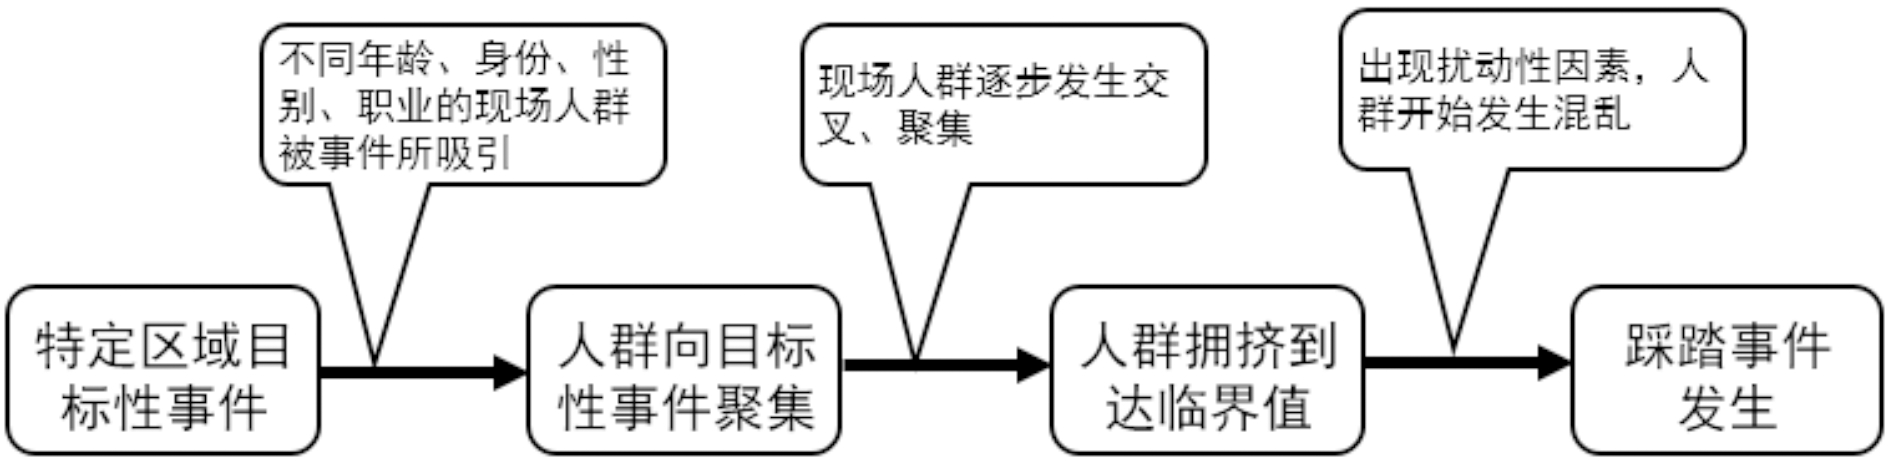
\includegraphics[scale=0.2]{img/stages.png}
	\caption{人群聚集事件的产生过程}
\end{figure}
我们的系统则可以根据以往的各方面数据、当前的手机信号数据、摄像头数据、网络舆论数据进行综合判断,保证实时反应城市中各个区域的人群阻塞情况,并尽量能指出将有可能产生危险的高危险区域,同时按照以往的经验给出建议。从而有助于城市管理人员及时发现并通过我们的系统向前线人员发送命令并且协调公安消防急救以及短信网络通知等其他社会职能部门以共同努力化解危机,在这些隐患给人民生产生活带来危险之前将它们消灭。我们的产品在整个过程中的角色可以如下图 \ref{fig:function} 所示。
\begin{figure}[H]
	\centering
	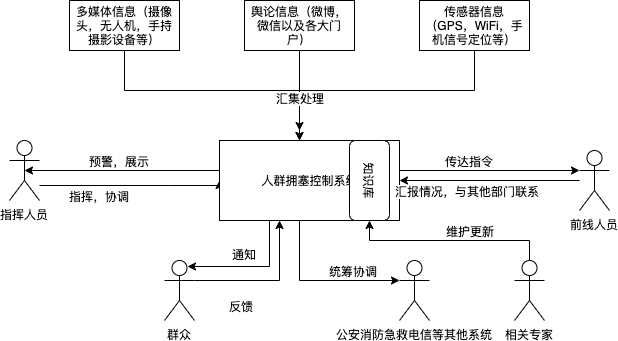
\includegraphics[scale=0.4]{img/function.png}
	\caption{\label{fig:function} 产品观点图}
\end{figure}

\section{产品功能}
如图 \ref{fig:process} 所示,我们的系统可以在事前预警、事中指挥部署以及事后进行记录。具体来说,我们的系统将根据视频信号、传感器信号以及网络舆论信号等汇总数据,与系统知识库进行分析比对之后向指挥人员给出相应等建议以及所需资源等等。之后指挥人员可以根据上述信息来联络相应的前线人员,向他们发送具体命令,并协调联系相关各方社会职能部门(比如公安消防以及急救电信等等)从而调动力量尽可能维持秩序并消灭可能的危险。在这个过程中,我们的系统呢将会记录各方的数据,从而可以用于后续的系统分析等等,以期系统可以不断进步。
\begin{figure}[H]
	\centering
	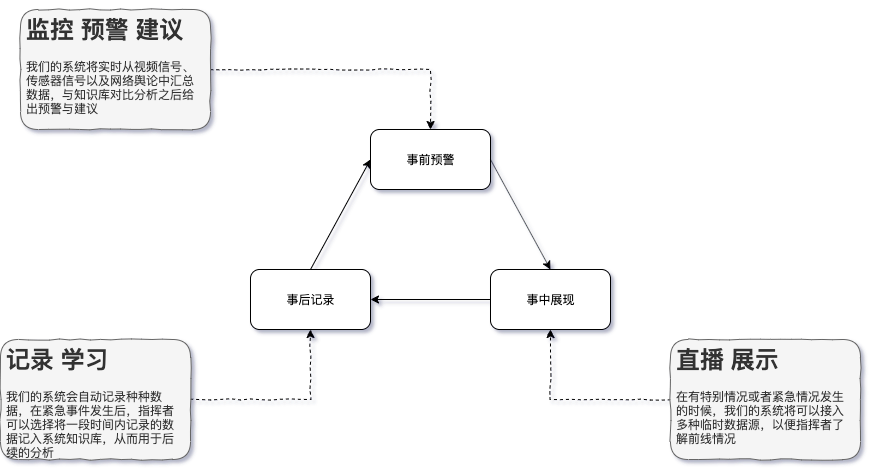
\includegraphics[scale=0.3]{img/process.png}
	\caption{\label{fig:process} 系统工作流程}
\end{figure}
\section{用户特征}
如图 \ref{fig:function} 所示,我们的系统用户主要分为六种,他们的主要特征以及在本系统中所期待的功能如下表所示。
\begin{longtable}{p{2cm}|p{10cm}}
\hline
用户 & 用户故事概要 \\
\hline
\hline
应急中心指挥人员 & 我希望能看到城市各地的人员密度分布,及时获取系统的预警信息,在事故发生时能和前线人员进行有效沟通,并获得网络舆情信息,事后还能管理事故的相关视频。\\
\hline
前线人员 & 我希望可以使用系统来接受指挥的指令,并与其他社会职能部门人员获得联络并查看目标地区的详细情况。除此之外,我还希望可以向指挥人员传输一线的直播数据以便他们了解情况。在完成工作之后,我还可以提交工作报告。\\
\hline
上级主管部门 & 我希望可以收到拥塞控制中心的报告并向其批示行动。 \\
\hline
公安急救公交交管电信部门 & 作为社会职能部门,我们希望可以获得来自拥塞控制中心的行动建议,并能反馈我们的行动方案,以便协助疏导人群拥塞事件。 \\
\hline
拥塞防控专家 & 作为拥塞防控专家,我希望可以通过已有案例建立案例库,通过提取抽象得到相应的策略库,资源库,以致于未来作参考。我希望可以通过输入事件特征快速检索知识库,给出解决问题的推荐方案以致于指导人员工作。\\
\hline
群众 & 群众主要分为受灾群众和其他群众,受灾群众迫切希望了解当前事态并获得专业的指导进行疏散;其他群众通过网络等方式报道实时状况,帮助专业人士和机构了解情况制定措施。\\
\hline
\caption{\label{tab:stakeholder} 利益相关者需求概要}
\end{longtable}
\section{系统约束}
如图 \ref{fig:function} 我们的系统受到以下的重要限制,他们对于我们的架构处理有极为重要的影响。
\begin{longtable}{p{2cm}|p{10cm}}
\hline
约束种类 & 约束内容 \\
\hline
\hline
 设备约束& 系统存储和处理能力都有限,无法处理全市所有的摄像头数据,仅能处理一部分已经预设好的重点区域的监控。\\
\hline
技术约束 & 人们有可能正在使用WIFI,有可能使用流量;有的人打开了GPS,有的人没有打开GPS,这可能使得最终得到的人员密度分布不全面。所以得结合三种定位技术获取到的信息来分析。\\
\hline
时间与预算约束& 按照项目要求,我们需要在四个工作月与项目预算内完成本次开发任务。 \\
\hline
用户约束 & 我们的用户种类很多,如指挥人员,前线人员,上级主管部门等,我们需要足够详尽的功能满足各方需求。\\
\hline
用户需求 & 因为部分使用者使用环境在户外,同时需要移动使用,所以系统应能实现移动外部访问。\\
\hline
技术约束 & 系统所需知识库模块需要使用自然语言处理机器模型,受现有技术约束,模型功能将会有所不足。\\
\hline
构建环境约束 & 开发团队成员分布在各个城市,同时磨合度不高,需要优秀的沟通协作工作工具提高开发效率。\\
\hline
\end{longtable}
\section{假设与依赖}
如下所示 我们系统的正常工作基于以下的重要假设:
\begin{itemize}
\item 监控中心能够建立起稳定可靠的数据中心,该中心与我们系统的各个外部组成部分保持良好的网络连接
\item 公安可以向我们开放摄像头的接入权限。
\item 监控中心与各主流社交网站、大众媒体建立充分的合作关系。
\item 运营商向我们开放基站定位权限,各大地图平台向我们提供WIFI辅助定位接口。
\item 信息部门拥有成熟的公众通知平台技术,可以及时在公众平台发布消息。
\item 知识库部门拥有合适的文本挖掘机器模型,可以有效抽象提取信息,拥有文本分词和向量化模型,可以将文本转化为数字进行比对。
\item 前线人员的设备拥有特殊的通信服务,从而保证加密和较大的带宽以保证通信。
\end{itemize}

\chapter{详细需求}
\section{外部接口}
\subsection{用户接口}
原型组
\subsection{其他系统接口}
我们的系统由于需要和多个外部系统共同工作,因此我们将会同多个外部系统共同配合工作,我们主要需要互动的外部系统有以下几个。
\begin{longtable}{p{2cm}|p{10cm}}
\hline
外部系统名 & 交互需求 \\
\hline
\hline
公安系统 & 本系统需要能向公安系统发送行动指导,并且从公安系统接受安排情况的回复 \\
\hline
急救系统 & 本系统需要向急救系统发送行动指导,并且从急救系统接受安排情况的回复 \\
\hline
公共交通系统 & 本系统需要向公共交通系统发送关于地铁公交车或者出租车的运行修改,以便可以避免人流的进一步涌入并协助从拥塞地点疏散人群 \\
\hline
交管局 & 本系统需要向交通管理局发送关于封路或者限流等等建议措施,从而有助于人流的快速疏散\\
\hline
电信公司 & 本系统需要向电信公司发送关于向特定区域内手机发送特定内容的信息,从而有助于群众了解情况或者帮助群众疏散 \\
\hline
上级主管部门 & 本系统可以向上级管理部门发送有关现在情况的说明以及准备采取的行动方案,由此上级部门可以作出决策并且向人群拥塞中心下达指令,以便拥塞控制中心获得相应权限。\\
\hline
\end{longtable}
\textbf{朋友们各自写自己需要的外部系统哈}

\subsection{硬件设备接口}
需要注意的是,我们的系统并不仅仅是一个软件系统,我们的系统还包括一些专门的硬件,它们主要是给前线人员所配备的专门设备(它们几乎都依赖与通信公司提供的特殊网络服务,从而保证安全性以及在人流量巨大的情况下仍然具有较高的带宽用于通信),我们对这些设备简述如下。
\begin{longtable}{p{2cm}|p{10cm}}
\hline
设备名 & 设备用途 \\
\hline
\hline
加密通信设备 & 前线人员使用加密通信设备来获取指挥人员下达的指令,与指挥人员相互发送信息以及语音对话。除此之外,在指挥人员对前线人员授权并发送相应信息之后,前线人员将可以通过本设备来和各种其他对职能部门进行对话(例如前线人员可以与来到前线的公安人员交流,并指挥他们协助人员疏散)。 \\
\hline
便携显示设备 & 前线人员使用便携显示设备来在获得授权的情况下查看指定区域内的摄像头直播或者查看一定区域内的人群拥塞热力图等等。 \\
\hline
摄像无人机 & 前线人员可以在前线放飞无人机,并将无人机所拍摄到的视频实时向指挥中心传送,以便指挥中心可以清楚的了解到现场的情况。 \\
\hline
手持摄像设备 & 前线人员可以在前线开启手持摄像设备,并且将拍摄到的视频与指挥中心进行直播,从而以便于指挥中心可以清楚的看到现场的情况。 \\
\hline
\end{longtable}
\textbf{朋友们各自写自己需要的硬件哈}
\section{功能性需求}
\subsection{指挥人员}
\subsection{前线人员}

\subsubsection{传递手持设备视频}
\begin{longtable}{p{2cm} | p{10cm}}
\hline
项目名 & 详述 \\
\hline
\hline
用例 & 传递手持设备视频 \\
\hline
主参与者 & 前线人员  \\
\hline
情景目标 & 向指挥部传递前线手持设备拍摄的视频,以便于指挥人员理解现场情况 \\
\hline
触发器 & 前线人员打开手持拍摄设备 \\
\hline
场景 & \begin{enumerate}
	\item 前线人员打开手持拍摄设备
	\item 前线人员配置网络连接
	\item 前线人员对重点地区进行拍摄,视频实时向指挥中心进行传递
	\item 完成传递之后前线人员关闭设备并断开连接
\end{enumerate} \\
\hline
参与者的连接渠道 & 手持拍摄设备 \\
\hline
\end{longtable}

\subsubsection{传递无人机视频}
\begin{longtable}{p{2cm} | p{10cm}}
\hline
项目名 & 详述 \\
\hline
\hline
用例 & 传递无人机视频 \\
\hline
主参与者 & 前线人员  \\
\hline
情景目标 & 向指挥中心传递前线无人机设备拍摄的实时画面从而使得指挥中心更好认识现场情况  \\
\hline
触发器 & 前线人员打开无人机 \\
\hline
场景 & \begin{enumerate}
	\item 前线人员打开无人机设备
	\item 前线人员设置连接信息
	\item 前线人员将无人机升空到适当的高度
	\item 无人机拍摄的视频实时向指挥中心进行传递
	\item 完成传递之后前线人员关闭设备并断开连接
\end{enumerate} \\
\hline
参与者的连接渠道 &  无人机\\
\hline
\end{longtable}

\subsubsection{查看所处区域附近摄像头视频}
\begin{longtable}{p{2cm} | p{10cm}}
\hline
项目名 & 详述 \\
\hline
\hline
用例 & 查看所处区域附近摄像头视频 \\
\hline
主参与者 & 前线人员  \\
\hline
情景目标 & 查看自己所处位置附近的摄像头列表并选取其中某个放大观看以便于了解附近的情况  \\
\hline
触发器 & 指挥中心给前线人员赋予权限 \\
\hline
场景 & \begin{enumerate}
	\item 前线人员使用显示设备查看自己权限范围中的各个摄像头视频的缩略视频
	\item 前线人员可以选中其中的某个摄像头并放大,从而更自仔细观看该摄像头的情况
	\item 前线人员使用完毕之后关闭显示设备
\end{enumerate} \\
\hline
参与者的连接渠道 & 显示设备 \\
\hline
\end{longtable}

\subsubsection{查看区域的综合热力图与拥塞情况分析}
\begin{longtable}{p{2cm} | p{10cm}}
\hline
项目名 & 详述 \\
\hline
\hline
用例 & 查看区域的综合热力图与拥塞情况分析\\
\hline
主参与者 & 前线人员  \\
\hline
情景目标 & 查看片区的人员聚集热力图以及拥塞情况报告从而判断地区中有拥塞可能的地区  \\
\hline
触发器 & 前线人员显示设备连接上线 \\
\hline
场景 & \begin{enumerate}
	\item 前线人员显示设备连接上线
	\item 前线人员查看到本地区的综合人流热力图以及各地的拥塞情况排名,其画面大概类似于指挥中心的情况
	\item 前线人员使用完毕之后关闭显示设备
\end{enumerate} \\
\hline
参与者的连接渠道 & 显示设备 \\
\hline
\end{longtable}

\subsubsection{查看或完成指挥人员派发的任务}
\begin{longtable}{p{2cm} | p{10cm}}
\hline
项目名 & 详述 \\
\hline
\hline
用例 &  查看或完成指挥人员派发的任务\\
\hline
主参与者 &前线人员  \\
\hline
情景目标 &查看或者点击完成指挥人员派发的任务队列以便于了解现阶段的主要任务  \\
\hline
触发器 & 指挥中心有新的任务发派给前线人员 \\
\hline
场景 & \begin{enumerate}
	\item 前线人员查看现在自己的任务列表
	\item 前线人员点击其中的最高优先级任务进行查看
	\item 前线人员在任务详情中可以看到该任务所要求的具体部署情况、其他各个部门的配合情况以及其他各个部门的工作人员的联系方式授权,以便前线人员可以通过系统来与他们沟通。
	\item 前线人员在完成任务之后可以选择「完成任务」
\end{enumerate} \\
\hline
参与者的连接渠道 & 加密通信设备\\
\hline
\end{longtable}

\subsubsection{与指挥人员发送信息}
\begin{longtable}{p{2cm} | p{10cm}}
\hline
项目名 & 详述 \\
\hline
\hline
用例 &  与指挥人员发送信息\\
\hline
主参与者 & 前线人员  \\
\hline
情景目标 &  与指挥人员发送信息并查看对方回复以便于与指挥人员交流看法 \\
\hline
触发器 & 前线人员有事物需要报告 \\
\hline
场景 & \begin{enumerate}
	\item 前线人员选择信息的等级与类型
	\item 前线人员输入信息的内容
	\item 如果需要前线人员还可以给该信息加入图片等文件
	\item 前线人员完成编辑之后点击发送,之后可以看到指挥人员的已读状态以及可能的回复
\end{enumerate} \\
\hline
参与者的连接渠道 & 加密通信设备 \\
\hline
\end{longtable}

\subsubsection{与指挥人员语音对话}
\begin{longtable}{p{2cm} | p{10cm}}
\hline
项目名 & 详述 \\
\hline
\hline
用例 & 与指挥人员语音对话 \\
\hline
主参与者 &  指挥人员\\
\hline
情景目标 &  与指挥人员进行语音对话以便于进一步交流看法或者做紧急部署\\
\hline
触发器 & 前线人员有事物要进行汇报\\
\hline
场景 & \begin{enumerate}
	\item 前线人员向指挥人员拨打通话
	\item 如果指挥人员接听,则可以开始对话,而且对话将会录音保存
	\item 如果到时指挥人员没有接听,则自动终止通话。
\end{enumerate} \\
\hline
参与者的连接渠道 &加密通信设备 \\
\hline
\end{longtable}

\subsubsection{提交工作报告}
\begin{longtable}{p{2cm} | p{10cm}}
\hline
项目名 & 详述 \\
\hline
\hline
用例 &  提交工作报告\\
\hline
主参与者 & 前线人员 \\
\hline
情景目标 &  在完成某些重大任务或者一定的时间期限之后向中心提交我的工作报告以期应急中心根据我的看法或者体会来充实知识库或者优化处理流程\\
\hline
触发器 & 前线人员完成某个任务之后\\
\hline
场景 & \begin{enumerate}
	\item 前线人员打开报告界面
	\item 前线人员对本次行动的各个方面进行评分
	\item 前线人员书写本次行动中认为自己做的好的以及不足的,以及认为各个部分好的以及不足的地方
	\item 前线人员提交报告
\end{enumerate} \\
\hline
参与者的连接渠道 & 加密通信设备\\
\hline
\end{longtable}

\subsubsection{与其他应急人员(公安消防急救等等)联络}
\begin{longtable}{p{2cm} | p{10cm}}
\hline
项目名 & 详述 \\
\hline
\hline
用例 & 与其他应急人员(公安消防急救等等)联络\\
\hline
主参与者 & 前线人员 \\
\hline
情景目标 &  在获得相应授权之后与同样获得指令来到前线的其他人员进行语音联络以便在前线协作指导各方工作\\
\hline
触发器 & 前线人员在指挥人员发出的任务或者信息中获得相应授权 \\
\hline
场景 & \begin{enumerate}
	\item 前线人员获得联系授权
	\item 前线人员选择要联系的部门,系统将会自动为他连线到被授权的该部门的工作人员的相应通信设备上
	\item 前线人员可以和他交流相应的问题
	\item 紧急事结束之后授权自动消失
\end{enumerate} \\
\hline
参与者的连接渠道 & 加密通信设备\\
\hline
\end{longtable}

\subsection{人群拥塞专家}
\subsection{上级主管部门}
\subsection{群众}
\subsection{公安急救公交交管电信部门}








\section{非功能性需求与系统质量属性}
李想
\section{设计约束}
\begin{longtable}{p{2cm}|p{10cm}}
	\hline
	设计约束种类 & 约束内容 \\
	\hline
	\hline
	语言类型& 系统使用JavaScript,Java,Python,SQL,HTML语言进行开发。\\
	\hline
	数据库 & 系统使用Mysql,Redis,Hive,Hbase数据库系统。 \\
	\hline
	时间范围 & 本次开发需要在四个工作月内完成。\\
	\hline
	测试 & 软件测试使用单元测试,集成测试,场景测试,功能测试,系统测试,Alpha测试,Beta测试。\\
	\hline
	错误跟踪 & 使用Backlog进行错误跟踪,更快地修复错误使团队记录和跟踪错误的过程更加容易。待办事项列表将报的问题变成清晰,易于遵循的轮廓,因此您可以更快地深入细节。\\
	\hline
	\end{longtable}
\chapter{附录}
\section{初步系统结构}
我们对系统进行了初步的分析与设计,得到了简要的系统物理结构图以及系统逻辑结构图分别如下所示。

我们的系统是一个典型的数据驱动型系统,我们的系统将可以从多个来源获得数据,而后由于网络通信能力的限制,我们将会使用边缘计算对数据进行一定对预处理,而后进行传输。之后我们对数据进行清洗和处理,而后经过我们的知识库对数据进行匹配监控,而后实时向拥塞控制中心的工作人员发布信息。指挥中心的人员将依赖于外部通信模块来完成于各个部门的信息交互于任务指派,从而尽可能快速的进行动员,尽可能将危险消灭于还未真正发生之时。
\begin{figure}[H]
	\centering
	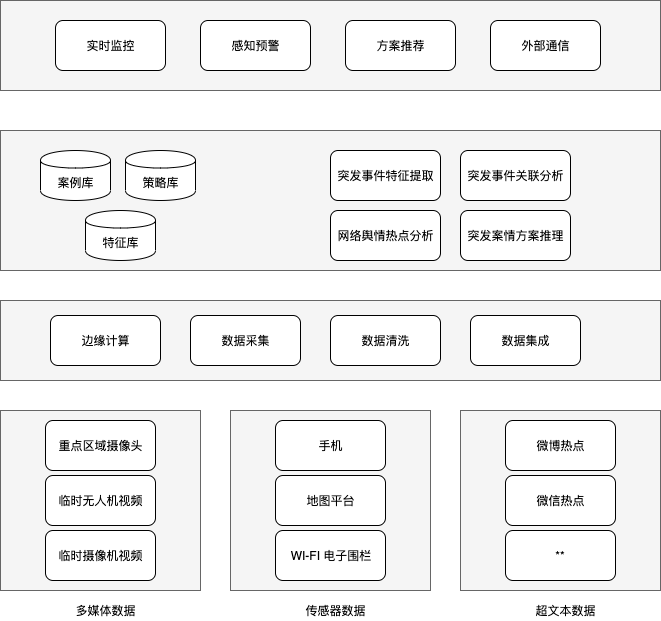
\includegraphics[scale=0.4]{img/logical.png}
	\caption{系统逻辑结构图}
\end{figure}

从我们的物理结构图将可以更加清楚的看出我们的系统将会从哪些数据源采集数据,我们的三大数据采集子系统(多媒体数据子系统、网络舆论数据子系统以及传感器子系统)堪称这个城市的神经系统,将会从这个城市的方方面面获取信息以用于分析处理,从而可以非常敏锐地发现问题并解决问题。
\begin{figure}[H]
	\centering
	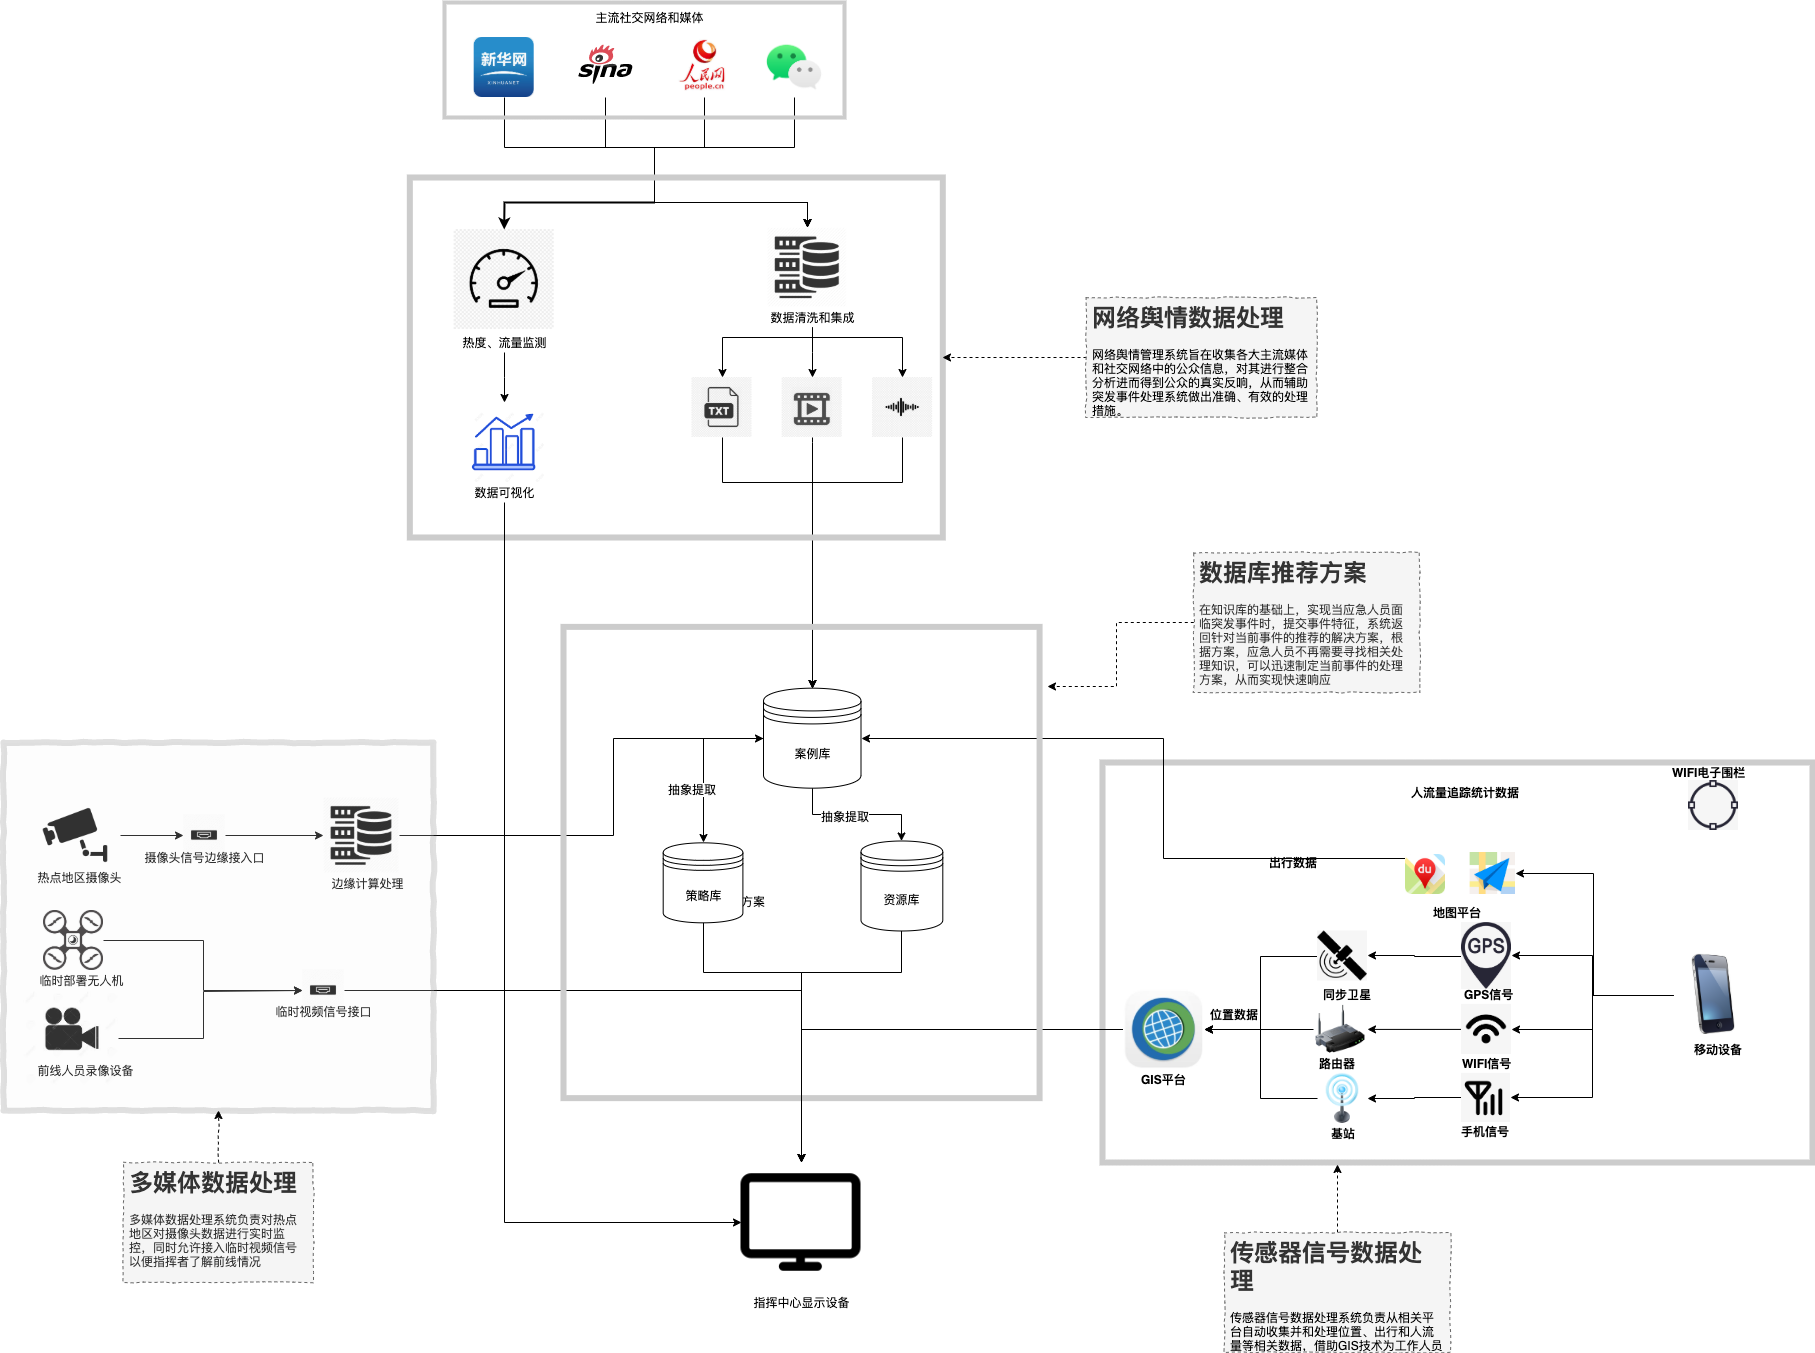
\includegraphics[scale=0.18]{img/physical.png}
	\caption{系统物理结构图}
\end{figure}
\section{需求工程概述}
我们的系统采用了一系列的需求工程方法来获取相应的需求,下面我们在这里简述我们的需求工程过程。
\subsection{需求诱导与分析}
我们采取了敏捷方法来获取本次项目的需求。首先,我们的组员同学分别扮演了一些本系统中的利益相关者,具体的利益相关者列表可以参看表 \ref{tab:stakeholder} 中的具体定义。我们可以看到,负责每一种角色的同学都会做一些调研,从而获取并整理出他们自己所负责角色的通常需求。而后我们使用微信电话召开了利益相关者会议,我们的项目经理认真的听取了各个利益相关者的意见,并把各方的需求汇总到了我们的「初步用户故事集」中(总计55个),具体可以参见附件中的Excel文件以及图 \ref{fig:team_story} 。在这个阶段我们主要采集的是系统的功能性需求,而系统的非功能性需求相对来说比较清晰,所以我们较快进行了汇总而没有包含在上述的用户故事集中。
\subsection{需求验证}
在完成了上述的需求诱导与分析之后,我们开始对现有的用户故事进行一定的拆分、合并和删除。比较明显的改变是有的时候某个利益相关者希望与系统的另一个利益相关者进行某种形式的通信,但是另一利益相关者并不知道有这样的请求,此时我们就要把这个故事进行补全,从而保证一致性。除此之外,我们有的用户故事的粒度太大了,我们很难在短期进行实现,因此我们把它们进行了拆分,分成一系列小的故事\footnote{例如我们的有一个用户故事是「指挥人员与各方交换信息」,我们就将其拆分为同具体每种被动参与者进行交流} 。另外,还有一部分用户故事实现难度过大,我们认为几乎不具有可行性,在这种情况下,我们选择直接取消这样的故事以保证系统用户故事的可实现性。

在进行了上述的处理之后,我们完成了初步的用例,并将它们整理出来,记录在本文档的详细需求规约当中。当然这个过程并不是一次就结束的,我们的利益相关者们在整个需求工程的过程中多次修改或者增加他们的用户故事,使得我们的需求工程成为一个典型的迭代的过程。
\subsection{需求管理}
为了保证我们的需求工程在不断的迭代过程中保持良好的可追溯性,我们使用了被广泛认可的软件项目管理工具     \href{https://www.teambition.com/}{Teambition} 来管理我们项目的需求。下面我们将展示一些我们使用需求管理工具尽心需求管理的截图。
\begin{figure}[H]
	\centering
	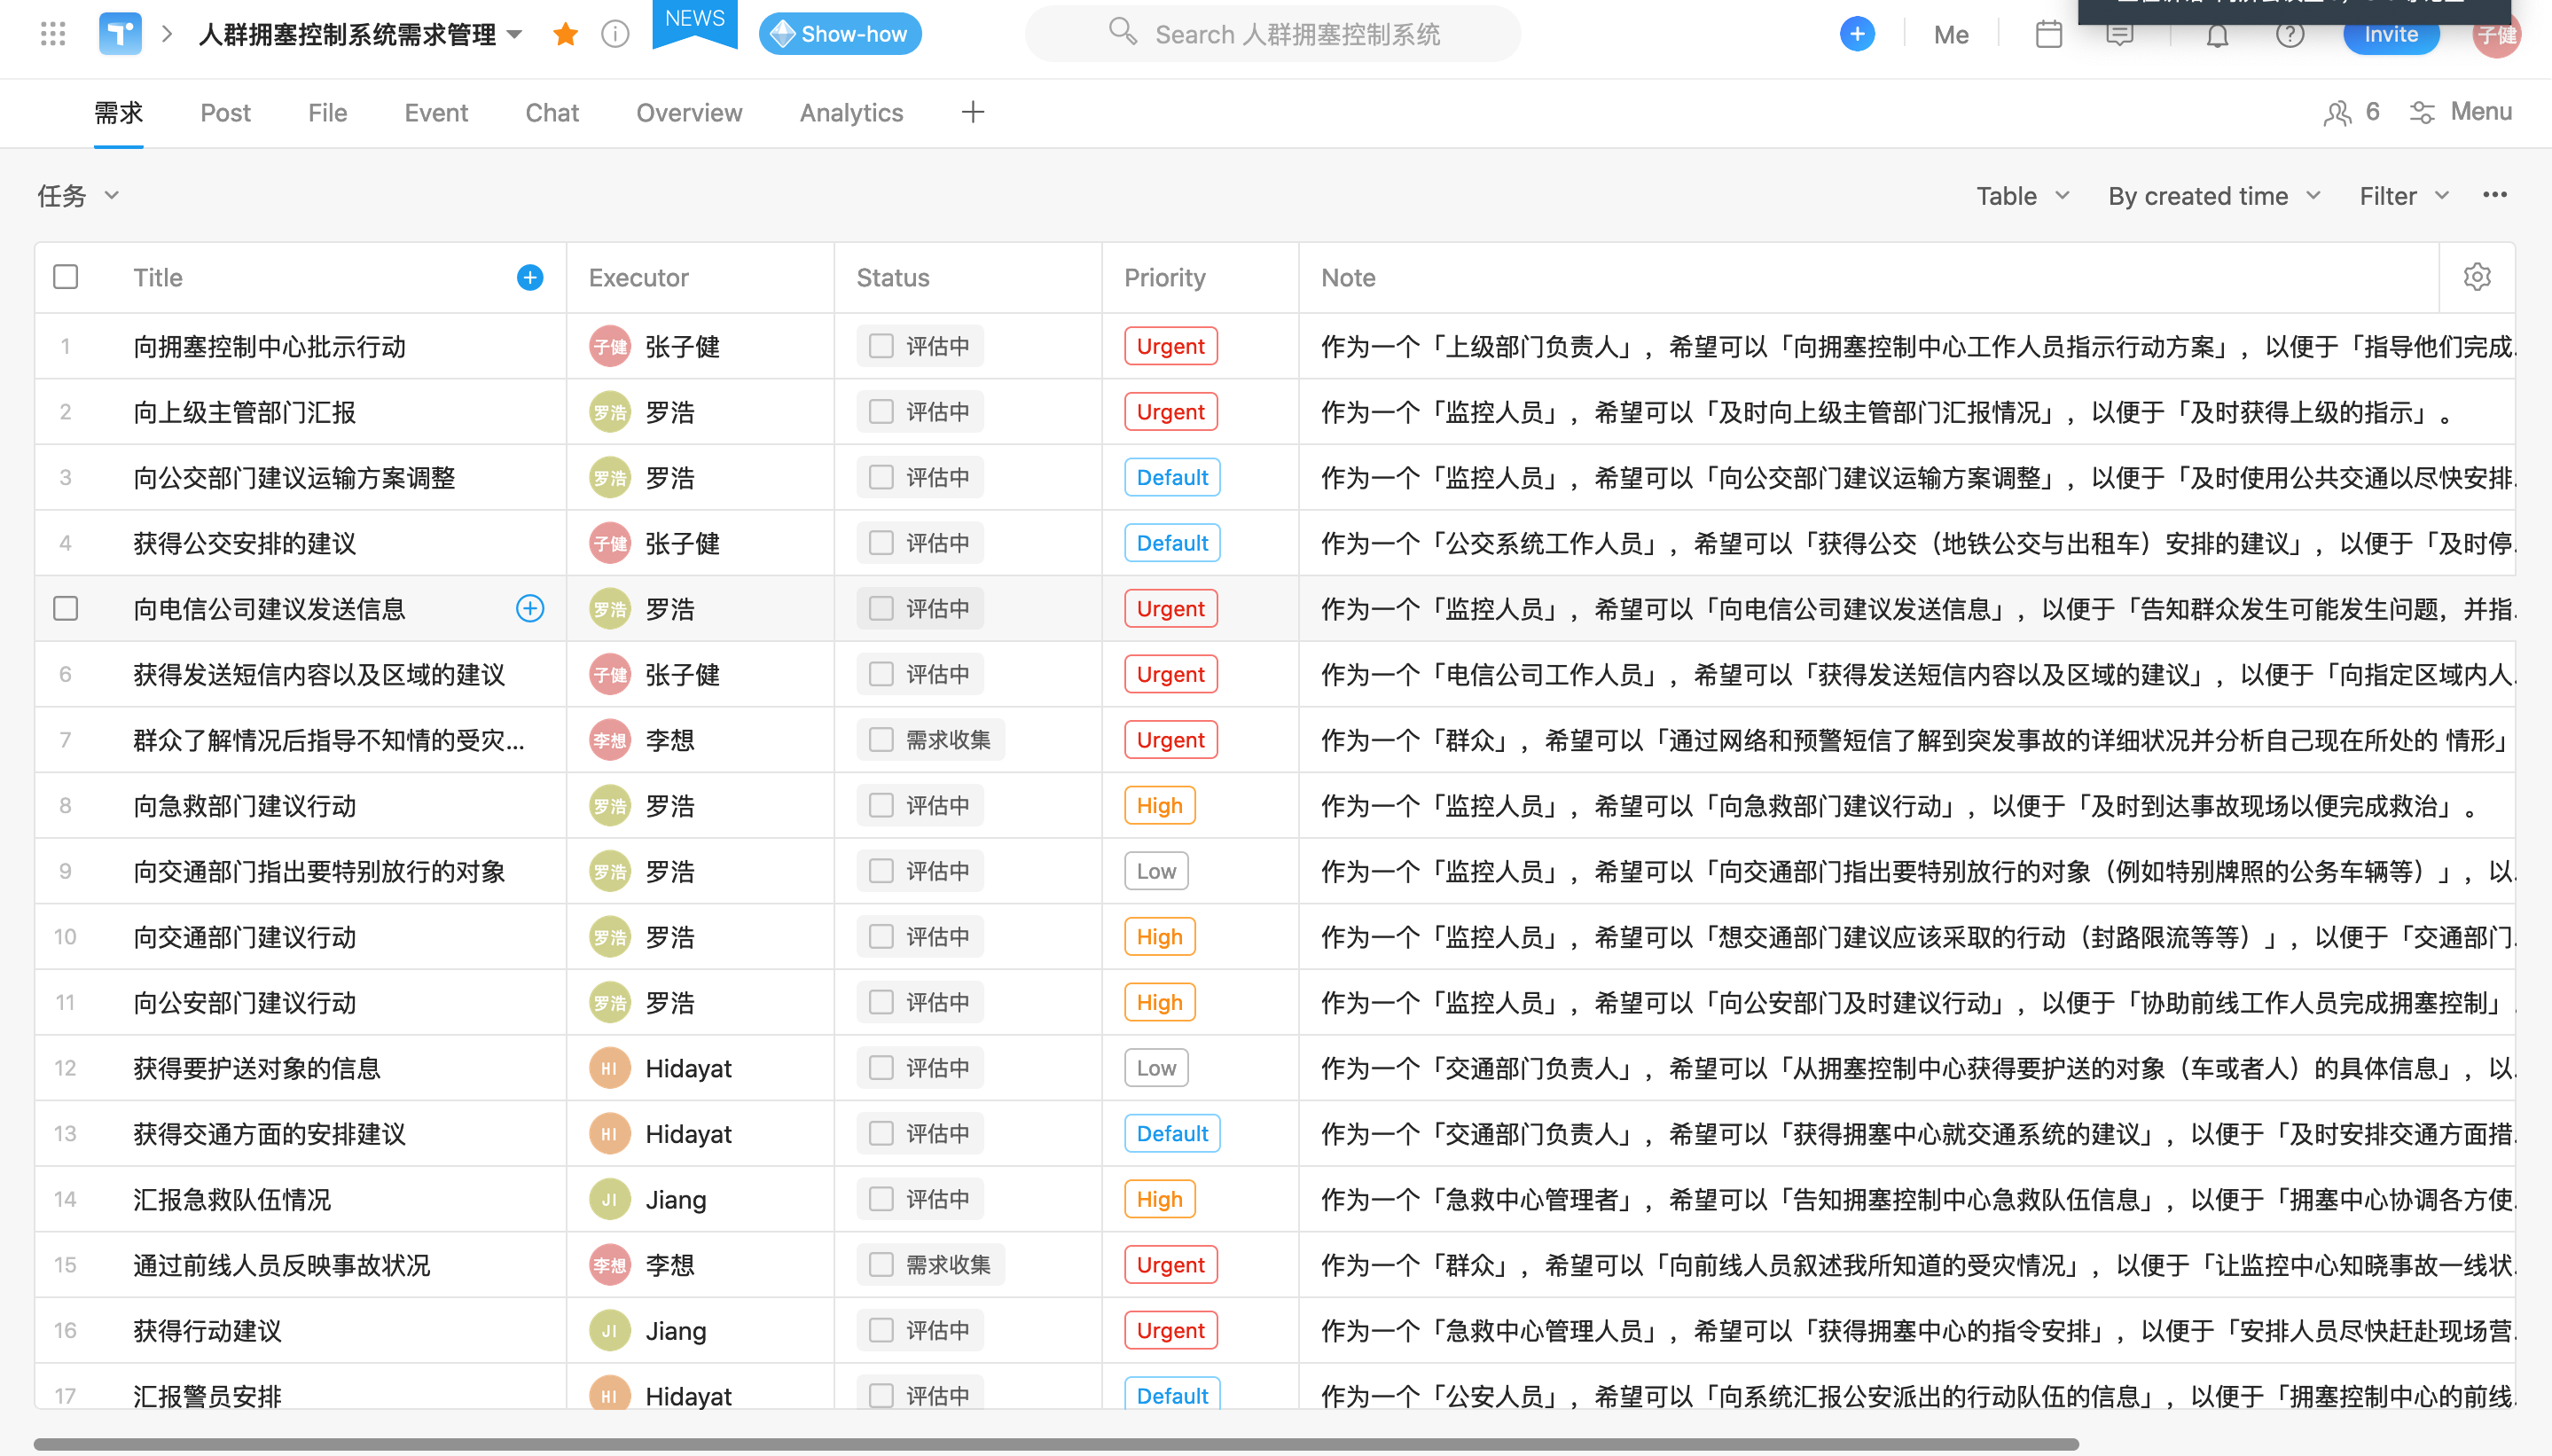
\includegraphics[scale=0.24]{img/userStory.png}
	\caption{\label{fig:team_story} 用户故事管理}
\end{figure}
上图 \ref{fig:team_story} 是我们进行用户故事管理的界面。每一个用户故事的具体情况都可以被分别追溯出来,如下图所示。我们可以看到有关这个用户故事的细节情况以及我们针对该用户故事进行修改的历史和交流的记录,这样我们可以非常清楚地看到我们的需求是怎么变化的。
\begin{figure}[H]
	\centering
	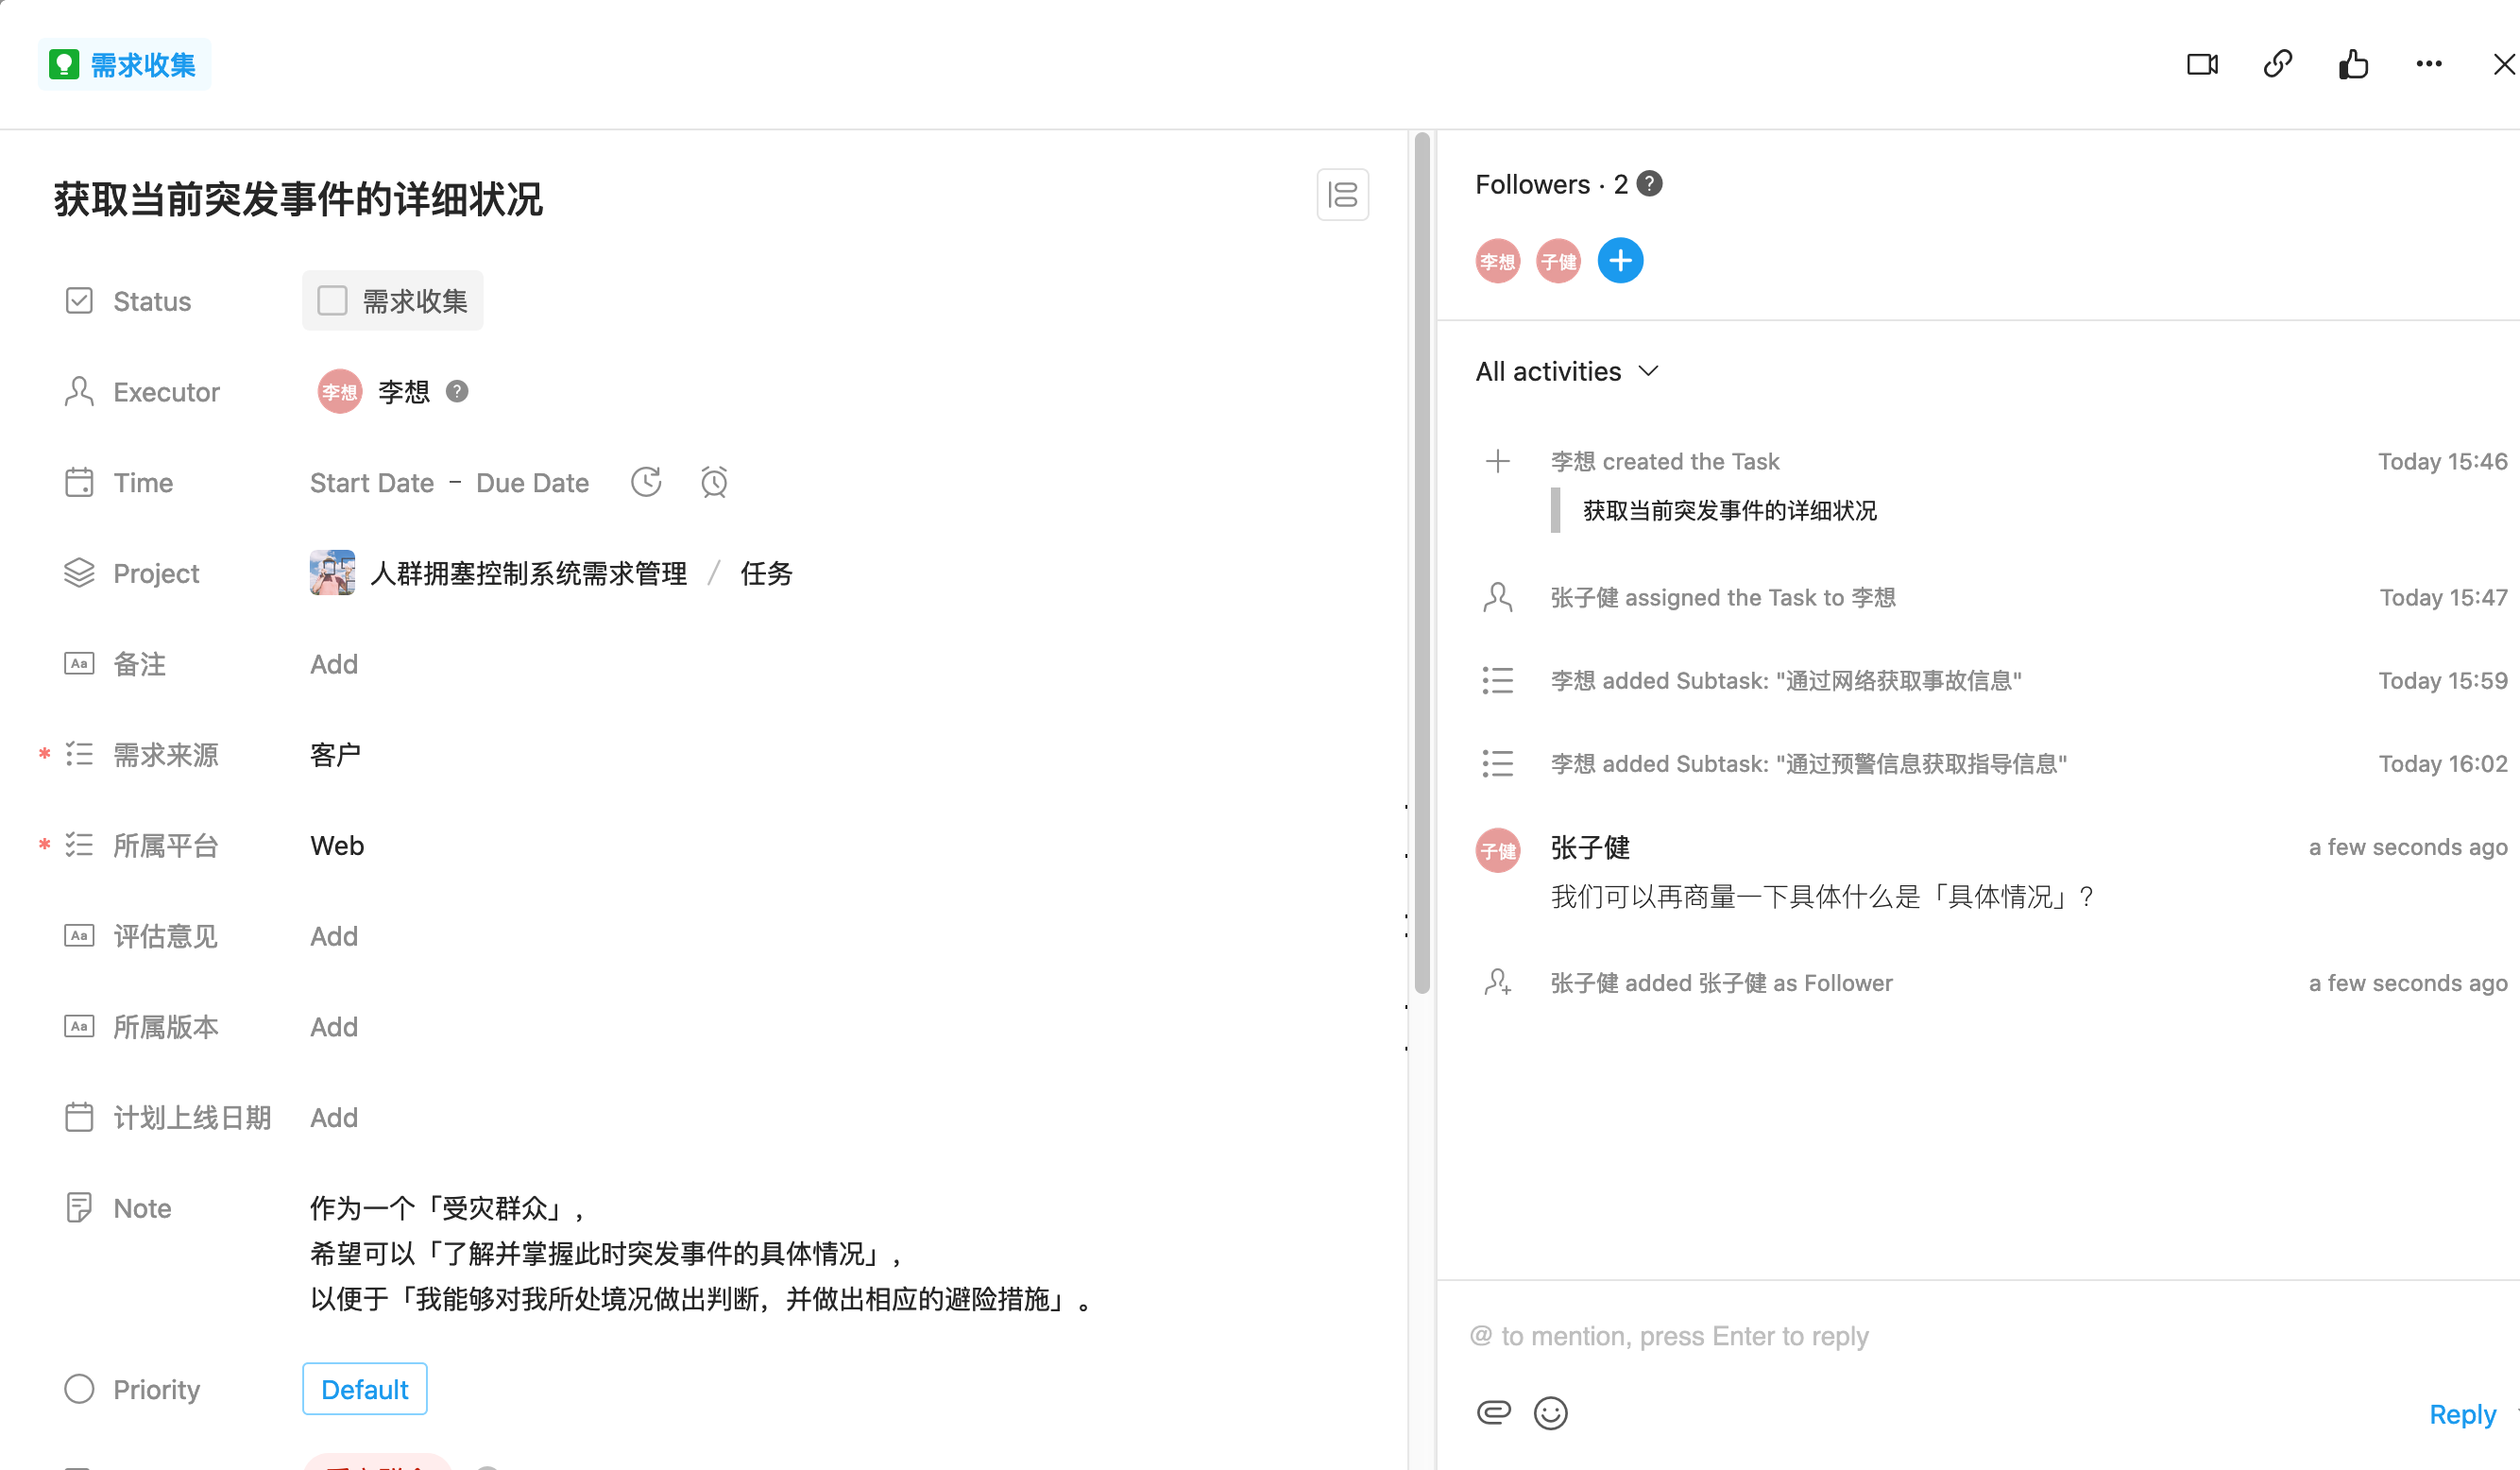
\includegraphics[scale=0.24]{img/storyDetail.png}
	\caption{\label{fig:story_detail} 用户故事修改细节}
\end{figure}
出去这样的常规内容,我们为了处理需求工程中这样一种尴尬的情况,既「每个利益相关者的用户故事是支离破碎的,我们怎么可以快速了解到该利益相关者整体的要求呢?」为了处理这个问题,我们加入了一些「长篇故事」,如下图所示。
\begin{figure}[H]
	\centering
	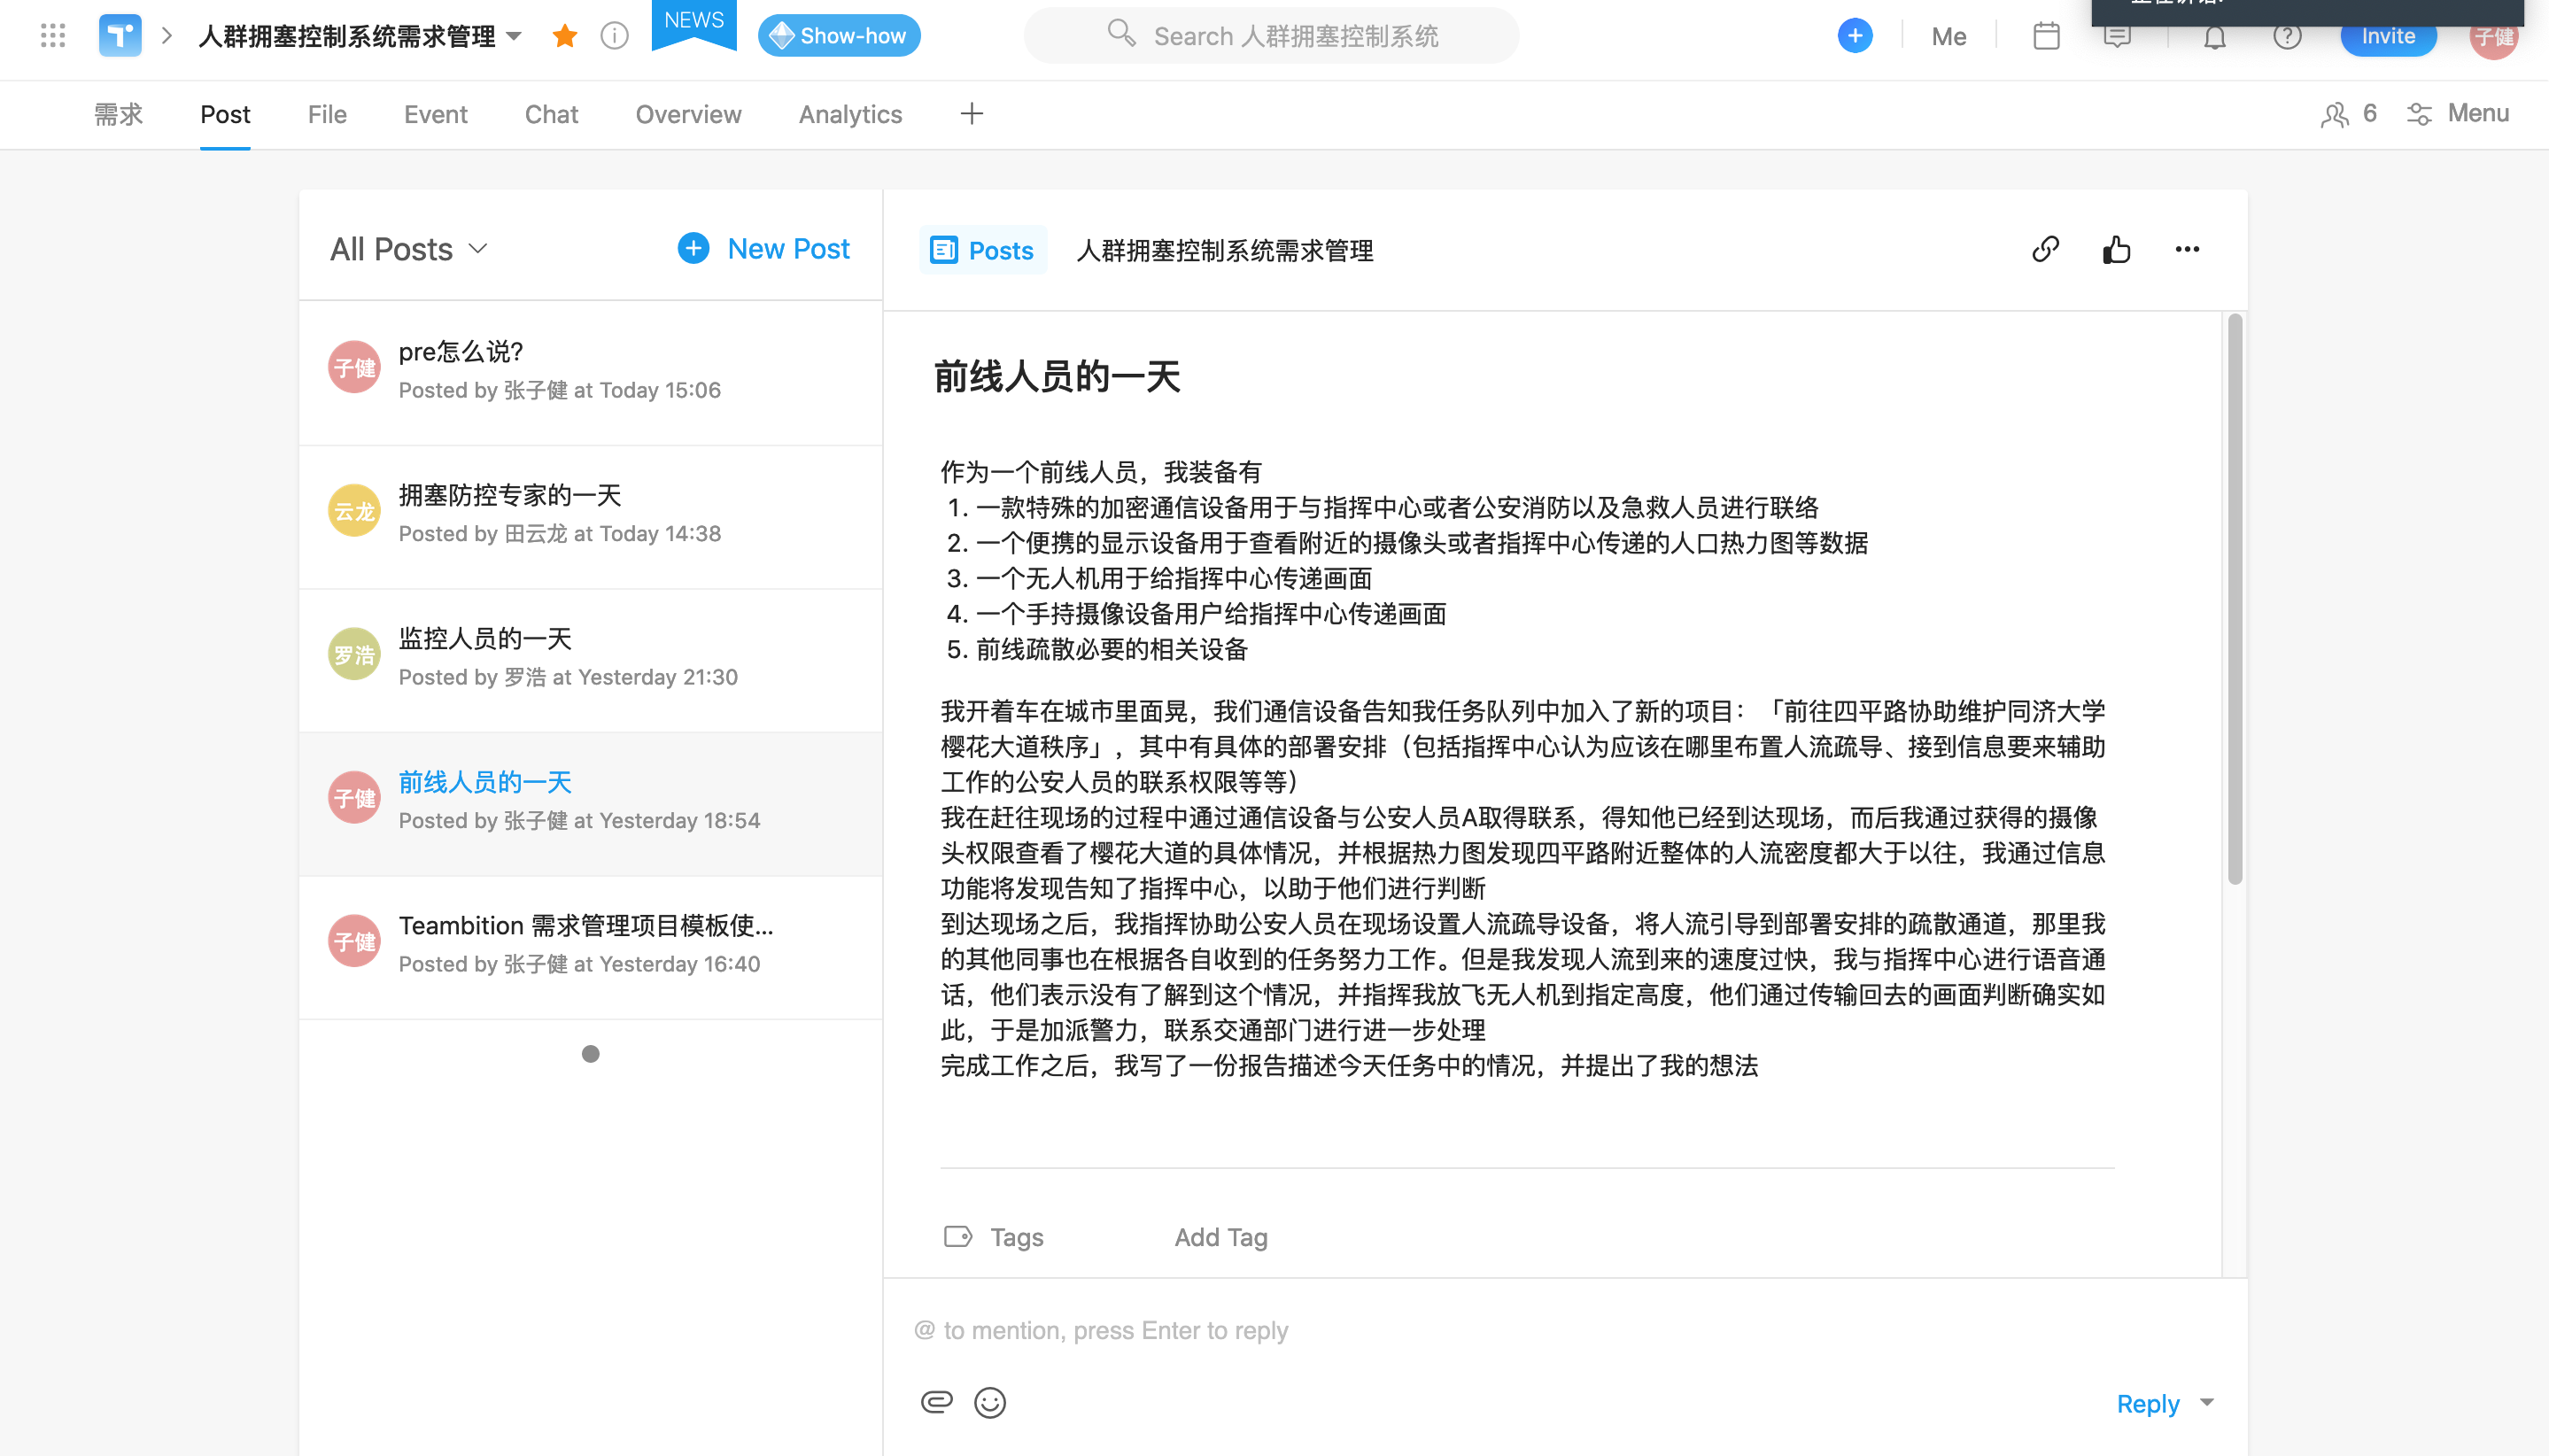
\includegraphics[scale=0.24]{img/longStory.png}
	\caption{\label{fig:long_story} 用户长故事}
\end{figure}
可以看到我们通过这样的长故事把较为复杂的用户的用户故事串联起来,这样我们各方就可以相对轻松的相互理解需求了。
\end{document}
